\chapter{Deformable Object Modelling}

One of the key challenges in manipulating deformable objects is the difficulty inherent in modeling and simulating them. While there has been some progress towards online modeling of deformable objects~\cite{Lang2002,Cretu2008} these methods rely on a time consuming training phase for each object to be modeled. This training phase typically consists of probing the deformable object with test forces in various configurations, and then fitting model parameters to the generated data. While this process can generate useful models, the time it takes to generate a model for each task can be prohibitive for some applications. Of particular interest are Jacobian-based models such as~\cite{Berenson2013} and~\cite{NavarroAlarcon2014}. In these models we assume that there is some function $\DeformMapping : \gripperCspace \rightarrow \reals^N$ which maps a configuration of $\ngrippers$ robot grippers $\gripperconfig \in \gripperCspace$ to a parameterization of the deformable object $\deformconfig \in \reals^N$, where $N$ is the dimensionality of the parameterization of the deformable object.  These models are then linearized by calculating an approximation of the the Jacobian of $\DeformMapping$:
\begin{align*}
    \deformconfig                               &= \DeformMapping(\gripperconfig) \\
    \frac{\partial \deformconfig}{\partial t}   &= \frac{\partial F(\gripperconfig)}{\partial \gripperconfig} \frac{\partial \gripperconfig}{\partial t} \\
    \deformvel                                  &= J(\gripperconfig) \grippervel \enspace .\numberthis
    \label{eqn:jacobian}
\end{align*}

\todoin{Remove/replace 'shared characteristic \dots tuned parameters'.}
Computation of an exact Jacobian $J(\gripperconfig)$ at a given configuration $\gripperconfig$ is often computationally intractable and requires high-fidelity models and simulators, so instead approximations are frequently used. A shared characteristic of these approximations is some reliance on tuned parameters. This tuning process can be tedious, and in some cases needs to be done on a per-task basis.

In this chapter we consider two types of approximate Jacobian models. The first approximation we use is a \textit{diminishing-rigidity Jacobian}~\cite{Berenson2013} which assumes that points on the deformable object that are near a gripper move ``almost rigidly'' with respect to the gripper while points that are further away move ``less rigidly''. This approximation uses deformability parameters to control how quickly the rigidity decreases with distance (Sec.~\ref{sec:diminishing_rigidity}). The second approximation we use is an \textit{adaptive Jacobian}~\cite{NavarroAlarcon2014} which uses online estimation to approximate $J(\gripperconfig)$. Adaptive Jacobian models rely on a learning rate to control how quickly the estimation changes from one timestep to the next (Sec.~\ref{sec:adaptive_jacobian}). In addition to Jacobian-based models, we also introduce a non-linear modification of the diminishing-rigidity Jacobian which more accurately captures the effect of the direction of gripper motion and obstacles (Sec.~\ref{sec:constrained_model}).

\section{Definitions}

Let the robot be represented by a set of $\ngrippers$ grippers with configuration $\gripperconfig \in \gripperCspace$.  We assume that the robot configuration can be measured exactly; in this work we assume the robot to be a set of free floating grippers; in practice we can track the motion of these with inverse kinematics on robot arms (see Sec~\ref{sec:stretching_avoidance_controller_physical_robot_implementation} for an implementation). We use the Lie algebra~\cite{Murray1994} of $\se3$ to represent robot gripper velocities. This is the tangent space of $\se3$, denoted as $\tanse3$. The velocity of a single gripper $\gripperidx$ is then $\grippervelG = \grippervelindiv \in \tanse{3}$ where $\transvelG$ and $\rotvelG$ are the translational and rotational components of the gripper velocity. We define the velocity of the entire robot to be $\grippervel = \grippervelexpanded \in \gripperVspace$. We define the inner product of two gripper velocities $\grippervel_1, \grippervel_2 \in \tanse3$ to be 
\begin{equation}
    \grippervelinnerprod = \grippervelinnerprodfull = \grippervelinnerprodexpanded \enspace,
\end{equation}
where $\rotvelweight$ is a non-negative scaling factor relating rotational and translational velocities. This defines the $\tanse3$ norm
\begin{equation}
    \grippervelGnormsq = \innerprod{\grippervelG}{\grippervelG}_\rotvelweight \enspace .
\end{equation}

Let the configuration of a deformable object be a set of $\ndeformpoints$ points with configuration $\deformconfig = \deformconfigexpanded \in \deformCspace$. We assume that we have a method of sensing $\deformconfig$. Let $\RelaxedDistMatrix$ be a symmetric $\ndeformpoints \times \ndeformpoints$ matrix where $\geodistIJ$ is the the geodesic distance (see Fig.~\ref{fig:geodesic}) between $\deformconfigI$ and $\deformconfigJ$ when the deformable object is in its ``natural'' or ``relaxed'' state. To measure the norm of a deformable object velocity $\deformvel = \deformvelexpanded \in \deformVspace $ we will use a weighted Euclidean norm
\begin{equation}
    \deformvelnormsq = \deformvelnormsqexpanded = 
\end{equation}
where $\Pinvweight = \Pinvweightexpanded \in \reals^\ndeformpoints$ is a set of non-negative weights. The rest of the environment is denoted $\obstacle$ and is assumed to be both static, and known exactly.

Let a \textit{deformation model} $\DeformForwardFn$ be defined as a function which takes as input the system configuration, gripper velocities, and obstacle configuration to a deformable object and returns a deformable object velocity:
\begin{equation}
    \deformvel = \DeformForwardFnFull \enspace .
\end{equation}
% \todo{Discuss quasi-static somewhere in here}
For brevity this will frequently be shortened to $\deformvel = \DeformForwardFn(\grippervel)$. For Jacobian based models, the basic formulation (Eq.~\eqref{eqn:jacobian}) directly defines the deformation model $\DeformForwardFn$
\begin{equation}
    \DeformForwardFn(\grippervel) = \JacobianFull \grippervel \enspace.
    \label{eqn:jacobianforwardfunction}
\end{equation}

\todoin{Deal with Eq.~\eqref{eqn:jacobian} and Eq.~\eqref{eqn:jacobianforwardfunction} vs. later (more correct) definition, and usage in section 3.2}

\todoin{Usage of $\tilde \DeformForwardFn$ and $\tilde \Jacobian$ throughout.}
\section{Approximate Jacobian Models}
\label{sec:jacobian_models}

Two use two different Jacobian approximation methods in this these; a diminishing rigidity Jacobian and an adaptive Jacobian, which are described below.

\subsection{Diminishing Rigidity Jacobian}
\label{sec:diminishing_rigidity}

The key assumption used by this method~\cite{Berenson2013} is \textit{diminishing rigidity}: the closer a gripper is to a particular part of the deformable object, the more that part of the object moves in the same way that the gripper does (i.e. more ``rigidly''). The further away a given point on the object is, the less rigidly it behaves; the less it moves when the gripper moves. This approximation depends on two parameters $\drktrans \geq 0$ and $\drkrot \geq 0$ which control how the translational and rotational rigidity scales with distance. Small values entail very rigid objects; high values entail very deformable objects.

For every point $\deformidx$ and every gripper $\gripperidx$ we construct a Jacobian $\Jrigid(\deformidx, \gripperidx)$ such that if $\deformconfigI$ was rigidly attached to the gripper $\gripperconfigG$ then
\begin{equation}
    \deformvelI = \JrigidIG \grippervelG = 
    \begin{bmatrix} \JtransIG & \JrotIG \end{bmatrix} \grippervelG \enspace .
\end{equation}
We then modify this Jacobian to account for the effects of \textit{diminishing rigidity}. Let the set of points grasped by gripper $\gripperidx$ be $\GraspedPointsFull \subseteq \deformconfig$. Then for 

Let $\closestpointIG$ be the index of the point with minimial relaxed geodesic distance to $\deformconfigI$ among the ones grasped by gripper $\gripperidx$:
\begin{equation}
    \closestpointIG = \argmin_{j \in }
\end{equation}

Let $\geodistIG$ be a measure of the distance between gripper $\gripperidx$ and point $\deformidx$. Then the translational rigidity of point $\deformidx$ with respect to gripper $\gripperidx$ is defined as
\begin{equation}
    \rigiditytransIG = e^{-\drktrans \geodistIG}
\end{equation}
and the rotational rigidity is defined as
\begin{equation}
    \rigidityrotIG = e^{-\drkrot \geodistIG}.
\end{equation}
To construct an approximate Jacobian $\tilde \Jacobian(\deformidx, \gripperidx)$ for a single point and a single gripper we combine the rigid Jacobians with their respective rigidity values
\begin{equation}
    \tilde \Jacobian(\deformidx, \gripperidx) = \begin{bmatrix} \rigiditytransIG \JtransIG & \rigidityrotIG \JrotIG \end{bmatrix} \enspace,
\end{equation}
and then combine the results into a single matrix
\begin{equation}
    \tilde \Jacobian(\gripperconfig, \deformconfig) = 
    \begin{bmatrix}
        \tilde \Jacobian(1,1) & \tilde \Jacobian(1,2) & \dots & \tilde \Jacobian(1, \ngrippers) \\
        \tilde \Jacobian(2,1) & \ddots \\
        \vdots \\
        \tilde \Jacobian(\ndeformpoints,1)
    \end{bmatrix} \enspace .
\end{equation}


\subsection{Adaptive Jacobian}
\label{sec:adaptive_jacobian}

A different approach is taken in~\cite{NavarroAlarcon2014}, instead using online estimation to approximate $\Jacobian(\gripperconfig, \deformconfig)$.
In this formulation we start with some estimate of the Jacobian $\tilde \Jacobian(0)$ at time $t = 0$ and then use the Broyden update rule~\cite{Broyden1965} to update $\tilde \Jacobian(t)$ at each timestep $t$
\begin{equation}
    \tilde \Jacobian(t) = \tilde J(t-1) + \ajrate \frac{\left( \deformvel(t) - \tilde \Jacobian(t-1) \grippervel(t) \right)}{\grippervel(t)^T \grippervel(t)} \grippervel(t)^T \enspace.
\end{equation}
This update rule depends on a update rate $\ajrate \in (0, 1]$ which controls how quickly the estimate shifts between timesteps.
\section{Constrained Directional Rigidity}
\label{sec:constrained_model}

\todoin{Update definitions to match formulation used here}
\todoin{Update notation used in this section}

\begin{figure}[t]
    \centering
    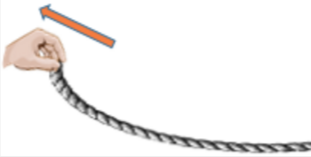
\includegraphics[width=.49\linewidth]{Intro_drag}\hfill
    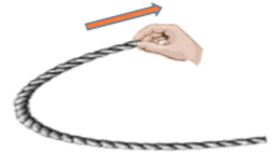
\includegraphics[width=.49\linewidth]{Intro_pull}%
    \caption{An illustrative example of directional rigidity. Left: The rope moves almost rigidly when dragging it by one end to the left. Right: The rope deforms when pulling it on the right in the opposite direction.}
    \label{fig:intro_directional_rigidity}
\end{figure}

While the diminishing rigidity Jacobian method has been used to do practical manipulation tasks with a deformable object with a precise physical model, we observe that this rigidity does not only diminish as the distance from the gripper increases. Instead, it is a function of a larger set of variables derived from the configuration of the object. The rigidity also depends on the direction of gripper motion. Fig.~\ref{fig:intro_directional_rigidity} shows an example of an object's \textit{directional rigidity}. In addition capturing the effects of directional rigidity, we seek to address contact with the environment, increasing the accuracy of $\tilde \DeformForwardFn$. 

\subsection{Geometric Model of Deformable Object Motion}

\subsubsection{Model Overview}
The approximate model locally describes the object's motion when given a motion of the grippers. Below we describe our approach first by specifying the model and then enforcing collision constraints on the prediction this model makes.

The current state of the deformable object is a function of the current gripper pose, the history of gripper motions that have been applied, the object's initial configuration, and the obstacles in the environment:

\begin{equation}
    \deformconfig = \DeformMappingExpanded
\end{equation}

To create a predictive model, we need to compute how $\deformconfig$ changes as a result of changing the gripper pose. Taking the time derivative of the above we obtain
\begin{equation}
\frac{d \deformconfig}{d t} = 
    \frac{\partial \DeformMapping}{\partial \gripperconfig}  \frac{\partial \gripperconfig}{\partial t} + 
    \frac{\partial \DeformMapping}{\partial \robotconfighist}\frac{\partial \robotconfighist}{\partial t} + 
    \frac{\partial \DeformMapping}{\partial \deformconfig_0} \frac{\partial \deformconfig_0}{\partial t} +
    \frac{\partial \DeformMapping}{\partial \obstacle}       \frac{\partial \obstacle}{\partial t}
\end{equation}

\todoin{Move this jacobian math definition up to the more generic math section.}
\noindent Only the first term is non-zero, thus
\begin{equation}
    \deformvel = \frac{\partial \DeformMappingExpanded}{\partial \gripperconfig} \grippervel
\end{equation}
$\frac{\partial \DeformMapping}{\partial \gripperconfig}$ is a matrix we call $\Jacobian$. In the previous section, $\Jacobian$ is assumed to be independent of $\grippervel$ and $\obstacle$, yielding\footnote{In this equation we replaced $\robotconfighist$ and $\deformconfig_0$ with $\deformconfig$, the current configuration of the object. $\robotconfighist$ and $\deformconfig_0$ are need in $\DeformMapping$ to compute the current state of the object, but if we can sense $\deformconfig$ directly (as we assume), then $\robotconfighist$ and $\deformconfig_0$ are not needed to compute $\tilde \Jacobian$.} $\frac{\partial \DeformMapping}{\partial \gripperconfig} = \Jacobian(\gripperconfig, \robotconfighist, \deformconfig_0) = \Jacobian(\gripperconfig, \deformconfig)$, which is analogous to a rigid-body Jacobian. While these assumptions allow a linear relationship between $\grippervel$ and $\deformvel$, and thus computational convenience, they are not accurate in many situations (see Figure \ref{fig:intro_directional_rigidity} for an example). In this section we change the definition of $\Jacobian$ to the following:

\begin{equation}
    \deformvel = \JacobianFull \grippervel = \DeformForwardFnFull
\end{equation}

We now describe how $\tilde \Jacobian$ is approximated, focusing on how it accounts for directional rigidity (using $\grippervel$) and how it enforces obstacle penetration constraints (using $\obstacle$).


\subsubsection{Directional Rigidity}
\todoin{Move parts that related to both diminishing rigidity and directional rigidity up a section}
\todoin{Go through and tie back to previous section}

We build on the idea proposed by Berenson~\cite{Berenson2013}, which approximates $\Jacobian$ based on the observation that the deformable object behaves rigidly near points grasped by the robot grippers. \cite{Berenson2013} encoded this effect through a simple function that only considered the distance of a point from the the nearest gripper. However, we find that we can exploit geometric information in the object's configuration to better predict the object's motion when we use a more complex model. We have observed that the key features of the deformable object configuration for predicting its motion are its deformability (which is determined by its material properties) and where it is slack. The deformation influences the transmission of the force from the grippers, i.e. the more stretchable the object, the more it will stretch when force is applied. However, when a region of the object is taut, regardless of how stretchable it is, it will move as if it were rigidly connected to a gripper (e.g. imagine a rope held taut by two grippers). We also must take into account that points are not influenced equally by different grippers, i.e. grippers farther away contribute less to the motion of a point than those closer to it.

\begin{figure}[t]
    \centering
    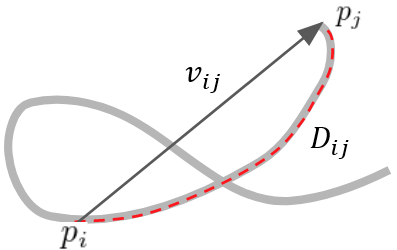
\includegraphics[width=1.5in]{method_geodesic.png}
    \caption{The length of the the red segment on the rope is the geodesic distance $\geodistIJ$. $\straightvecIJ$ is the vector showing the relative position of $\deformconfigJ$ with respect to $\deformconfigI$.}
    \label{fig:distance_vec_defs}
\end{figure}

To incorporate the above effects into our model, we define the following variables, which can be derived from $\gripperconfig, \grippervel$, and $\deformconfig$:
\begin{itemize}
    \item $\geodistIJ$: the geodesic distance (a scalar) between points $\deformconfigI$ and $\deformconfigJ$ on the surface of the object.
    \item $\straightvecIJ$: the vector starting at a point $\deformconfigI$ and ending at the point $\deformconfigJ$, as shown in Fig.~\ref{fig:distance_vec_defs}.
    \item $\gripperconfigG$: the configuration of gripper $\gripperidx$.
    \item $\grippervelG$: the velocity of gripper $\gripperidx$.
\end{itemize}

Furthermore, let $\closestpointIG$ be the index of the point with the minimal geodesic distance to $\deformconfigI$ among the ones grasped by the $\gripperidx$'th gripper. We address the notion of rigidity in object motion by considering the slackness of the object and reformulating the rigidity as a function of $\geodistIG$, $\straightvecIG$, and $\grippervelG$. For each point $\deformidx$ and gripper $\gripperidx$ we compute
\begin{equation}
\begin{split}
    \tilde \Jacobian(\deformidx, \gripperidx) 
                        &= \influenceIG \begin{bmatrix} \rigiditytransIG \JtransIG & \rigidityrotIG \JrotIG \end{bmatrix} \\
    \rigiditytransIG    &= \rigiditytrans(\geodistIG, \straightvecIG, \grippervelG) \\
    \rigidityrotIG      &= \rigidityrot(\geodistIG) \\
\end{split}
\label{eq:trans_rot_rigidity_diminishing_jacobian}
\end{equation}
$\rigiditytrans$ and $\rigidityrot$ are the corresponding translational and rotational diminishing rigidity factors defined by $\deformconfigI$ and gripper $\gripperidx$ (discussed below). 

Our goal is to encode the directional rigidity of the object motion into $\rigiditytrans$ and $\rigidityrot$ and use $\influenceIG$ to describe the \textit{influence} of gripper $\gripperidx$ on $\deformconfigI$. Intuitively, $\rigiditytrans$ should decrease with the increasing geodesic $\geodistIG$ distance between $\deformconfigI$ and $\deformconfig_{\closestpointIG}$. This is because the deformation of the region between $\deformconfigI$ and $\deformconfig_{\closestpointIG}$ will attenuate the transmitted force of the gripper's motion unless the object is taut. Since the effects on $\rigidityrotIG$ from $\grippervelG$ and $\straightvecIG$ are not as clear or significant as $\geodistIG$, we keep $\rigidityrotIG$ as a function of $\geodistIG$, where 
\begin{enumerate}
    \item $\rigidityrotIG$ ranges between $0$ and $1$.
    \item $\rigidityrotIG$ decreases as $\geodistIG$ increases.
\end{enumerate}
We give the definition of $\rigidityrotIG$ below.

From observation, we find two key reasons related to the slackness of the object that induce the diminishing rigidity effect for translation motion, and we aim to encode these factors into $\rigiditytransIG$. The first case is that the moving direction of $\grippervelG$ makes the region on the object between $\deformconfigI$ and $\deformconfig_{\closestpointIG}$ less taut. The second case is that this region is already slack. $\rigiditytransIG$ is thus a product of two terms:
\begin{equation}
    \rigiditytransIG = \tensionIG \slackIG
    \label{eq:Combined_directional_rigidity}
\end{equation}
where $\tensionIG$ addresses the effect in the first case (motion reducing tension), and $\slackIG$ addresses the effect in the second case (object slackness). Both $\tensionIG$ and $\slackIG$ are functions of some of $\gripperconfigG, \grippervelG, \deformconfigI$, or variables derived from these.

For $\deformconfigI$ on the object, we find $\tensionIG$ is greatly impacted by $\straightvecIG$ and $\transvelG$. Decomposing $\transvelG$ into $\transvelGRad$, the component in the direction of $\straightvecIG$, and $\transvelGPerp$, the component perpendicular to $\straightvecIG$. We observed that if $\transvelGRad$ is in the opposite direction to $\straightvecIG$, then it is more likely to make the intervening region slacker and thus reduce the transmission of force from the gripper to $\deformconfigI$. Moreover, if $\transvelGRad$ and $\straightvecIG$ are in the same direction when the object is not already slack, $\deformconfigI$ can move almost rigidly with $\grippervelG$. Fig.~\ref{fig:intro_directional_rigidity} shows an example of the impact of this alignment. Based on these observations, we design the function $\tensionIG = \tensionIGfull$ with the following properties:
\begin{enumerate}
    \item $\tensionIGfull$ ranges between $0$ and $1$.
    \item $\tensionIGfull > \tensionJGfull$
        \textbf{if} $\innerprod{\straightvecIG}{\transvelG} > \innerprod{\straightvecJG}{\transvelG}$
        \textbf{and} $\geodistIG = \geodistJG$.
    \item $\tensionIGfull > \tensionJGfull$
        \textbf{if} $\innerprod{\straightvecIG}{\transvelG} = \innerprod{\straightvecJG}{\transvelG}$
        \textbf{and} $\geodistIG > \geodistJG$.
\end{enumerate}
We give the definition of $\tensionIGfull$ below.


As mentioned above, $\slackIG$ depends on the current slackness of the intervening region. Without other external forces applied on the object, the pulling force applied by the robot will tend to unwind or unfold the object eventually (we do not consider cases where the object is tied into knots). For this reason,  the part of the intervening region on the object that is not already spread out is less likely to move rigidly with gripper $\gripperidx$. One indicator that can address this property is the ratio between the Euclidean distance between $\deformconfigI$ and $\deformconfig_{\closestpointIG}$, and the geodesic distance $\geodistIG$ between them. We denote $\distratioIG = \frac{||\straightvecIG||}{\geodistIG}$ to be this ratio. A larger $\distratioIG$ indicates a tauter intervening region. A tauter intervening region is more likely to result in $\deformvelI$ moving more rigidly. Thus we can design the function $\slackIG = \slackIGfull$ with the following properties:
\begin{enumerate}
    \item $\slackIGfull$ ranges between $0$ and $1$.
    \item $\slackIGfull = 1$ if $\distratioIG = 1$.
    \item $\slackIGfull > \slackJGfull$ if $\distratioIG > \distratioJG$
\end{enumerate}

Finally, $\influenceIG$, which captures the influence of gripper $\gripperidx$ on $\deformconfigI$ should have the following property (where $k$ is the index of a different gripper on the robot):
\begin{enumerate}
    \item $\influenceIG$ ranges between $0$ and $1$.
    \item $\influenceIG < \influenceIK$ if $\geodistIG > \geodistIK$.
    \item $\sum_{m = 1}^{\ngrippers} \influenceIM = 1$.
\end{enumerate}

\todo{Confirm that $\influenceIG$ has these properties.}


Through experimentation, we obtained good results with the following functions:
\begin{equation}
\begin{split}
    \tensionIGfull  &= e^{\drkdir \geodistIG \left(\cos \angle \left( \straightvecIG, \transvelG \right) - 1\right)} \\
    \slackIGfull    &= \left( \frac{\| \straightvecIG \|}{\geodistIG} \right) ^{\drkdist} \\
    \rigidityrotIG  &= e^{-\drkrot \geodistIG} \\
    \influenceIG    &= \frac{x_\gripperidx}{\sum_{m = 0}^\ngrippers x_m}\\
    x_m             &= \frac{\textrm{min} \{\geodistI{1}, \dots , \geodistI{\ngrippers}\}}{\geodist_m} 
\end{split}
\label{eq:directional_rigidity_factors}
\end{equation}
where $\drkdir$, $\drkdist$, and $\drkrot$ are non-negative parameters. Specifically, a larger $\drkdir$ indicates a greater impact on the diminishing in the rigidity from the motion reducing tension. A larger $\drkdist$ indicates a greater impact on the diminishing in the rigidity from the slackness of the object in the current state. A larger $\drkrot$ indicates a faster decrease in rotational rigidity as the distance from $\deformconfigI$ to the gripper increases. 
\todo{Confirm no negative before $\drkdir$ in Eq.~\eqref{eq:directional_rigidity_factors}}


\begin{figure}
    \centering
    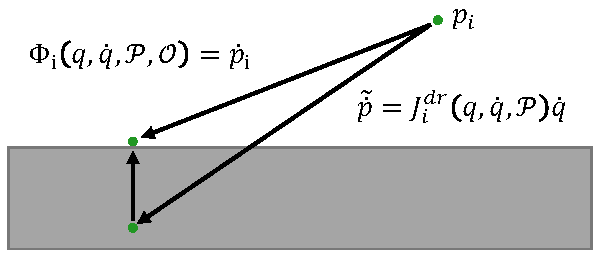
\includegraphics[width=3in]{point_projection}
    \caption{Projection process for points that are predicted to be in collision after movement.}
    \label{fig:point_projection}
\end{figure}

\subsubsection{Obstacle Penetration Constraints}

By combining the contributions of each individual gripper using the model developed above, we get a prediction of a point's movement from
\begin{equation}
    \approxPVI = \begin{bmatrix}
        \Jacobian(\deformidx, 1) & \dots & 
        \Jacobian(\deformidx, \ngrippers)
    \end{bmatrix} \grippervel = \Jacobian_{\deformidx}(\gripperconfig, \grippervel, \deformconfig) \grippervel
\end{equation}
However, at this stage, we haven't take into account the effect from the obstacles $\obstacle$. Thus the predicted $\approxPVI$ can move $\deformconfigI$ into an obstacle.

When the prediction of $\deformconfigI$ enters the obstacle, we project any penetration by the predicted $\approxPVI$ into the tangent space of the obstacle surface (Fig.~\ref{fig:point_projection}). Let $d_\deformidx < \| \approxPVI \|$ be the distance to collision in direction $\approxPVI$ from point $\deformconfigI$; let $\lambda_\deformidx = \frac{d_\deformidx}{\| \approxPVI \|}$; let $n_\deformidx$ be the unit surface normal of the obstacle in contact; and let $N_\deformidx = (\eye_{3\times 3} - \vec{n}_\deformidx \vec{n}_\deformidx^+)$. Then to account for obstacles we compute
\begin{equation}
    \tilde \Jacobian_\deformidx(\gripperconfig, \grippervel, \deformconfig, \obstacle) =
    \begin{cases}
        (\lambda_\deformidx + (1 - \lambda_\deformidx)N_\deformidx) \Jacobian_\deformidx(\gripperconfig, \grippervel, \deformconfig) & \text{if $\deformconfigI + \approxPVI$ in collision} \\
        \Jacobian_\deformidx(\gripperconfig, \grippervel, \deformconfig) & \text{otherwise}
    \end{cases}
\end{equation}
To generate $\Jacobian$ for all the points and grippers we compute $\Jacobian_\deformidx(\gripperconfig, \grippervel, \deformconfig)$ for each $\deformconfigI$. These matrices are modified using penetration constraints to get $\Jacobian_\deformidx(\gripperconfig, \grippervel, \deformconfig, \obstacle)$. These matrices are then stacked to obtain $\Jacobian(\gripperconfig, \grippervel, \deformconfig, \obstacle)$. Finally, we arrive at our approximate model: $\DeformForwardFnFull = \JacobianFull \grippervel$.
\subsection{Results}
\label{sec:stretching_constraint_controller_results}

Our goal for this new controller is formulating a set of constraints for the controller to mitigate collision and excessive stretching issues. As mentioned in previous sections, our benchmark controller is based on \cite{Berenson2013} and described in Sec.~\ref{sec:stretching_avoidance_controller}. To evaluate our method we perform experiments in simulation and on a physical robot. The simulator used is Bullet physics \cite{Coumans2010}, however, we emphasize that our method has no knowledge of the simulation parameters or simulation methods used therein. The simulator is used as a ``black-box,'' mainly to stand in for a perception system and to allow us to do repeatable experiments. The physical robot consists of two KUKA iiwa 7DoF arms with Robotiq 3-finger hands.

\todoin{Separate text/wording etc. for model vs controller.}

We ran experiments with scenarios involving both cloth and rope. The parameters are set as $\drkdir = 4$, $\drkdist = 10$, $\drkrot = 20$ for the new model, $l_c = 0.023$, and $s_s = 0.4$ for the new controller. The parameters we used for the benchmark method are its default best value found in \cite{McConachie2018}. The stretching detection ratio is set as $\stretchmax = 1.667$ for the cloth and $\stretchmax = 1.1$ for the rope. The maximum gripper motion is set as $grippervelmaxservo = 0.2$. For the experiment with a task goal defined, a precalculated Dijkstra field for the task will generate the $\deformvel_e$ for each point at each state to move the object toward the goal given each point's current position in the space as described in Sec.~\ref{sec:reducing_error}. All experiments were run on a i7-8700K 3.7 GHz CPU with 32 GB of RAM. A video showing the experiments is included with this paper.


\subsection{Constraint Enforcement}
\label{Results: Object Stretching Avoidance}

Since the benchmark controller can already handle the collision constraint very well, and the new controller addresses the collision constraint in the similar way as the benchmark, there is not a significant difference in how the collision constraint is enforced. However, the stretching constraint shows a very clear improvement.

The metrics of stretching avoidance is the stretching ratio $\stretchcurr$ defined in Section \ref{Method_Overstretch}. A controller with good stretching avoidance should prevent $\stretchcurr$ from increasing beyong a certain threshold.

The two experiments we used for the stretching avoidance test are the rope-wrapping-cylinder and the cloth-passing-single-pole, shown in Fig.\ref{fig:experimental_setup_scene} (left column). We ran each controller separately for a fixed amount of time for each task and show $\stretchcurr$ vs. time for both controllers in Fig. \ref{fig:experiment_stretching_factorFig: experiment_stretching_factor}. In both these two setups, the desired object motion $\deformvel_e$ generated by the Dijkstra field will tear the object unless overstretching is prevented.%, thus the 

Fig. \ref{fig:experiment_stretching_factorFig: experiment_stretching_factor} shows the new controller is able to prevent further stretching happening when the object is taut for both the rope and the cloth. In the rope test, the new controller can prevent overstretching with $s_s = 0.4$, as defined in Eq.\ref{Eq: Stretching_avoidance_Method_This_Paper}. We can see the $\stretchcurr$ of the benchmark methods keeps growing beyond this threshold, while the $\stretchcurr$ of the new method stays close to the threshold. In the cloth test, the benchmark method's $\stretchcurr$ (in purple) increases above the threshold $\stretchmax = 1.667$ for cloth, and a sudden drop in $\stretchcurr$ happens after running the test for $2$ seconds. This drop is the ``tearing'' point in the simulator. Though we still see overstretching happened using the new method for some settings of $s_s$, in all cases the $\stretchcurr$ converged before tearing happened (instead of growing without bound). 

\begin{figure}[t]
    \centering
    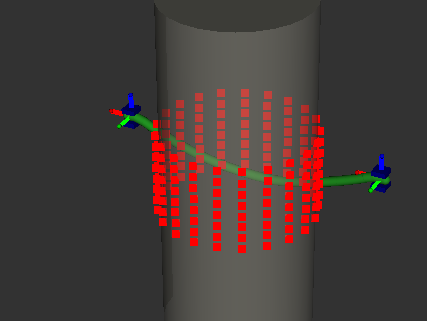
\includegraphics[width=.45\linewidth]{rope_cylinder}\hfill
    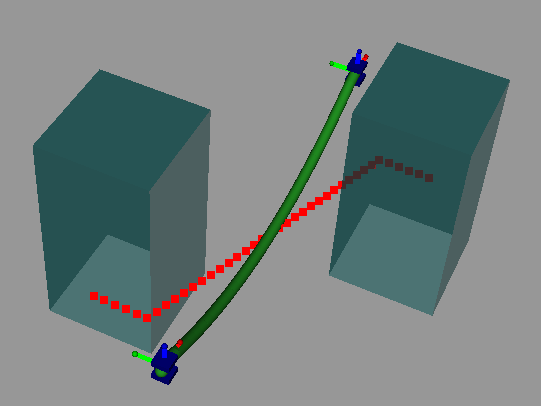
\includegraphics[width=.45\linewidth]{rope_zig_match}\\
    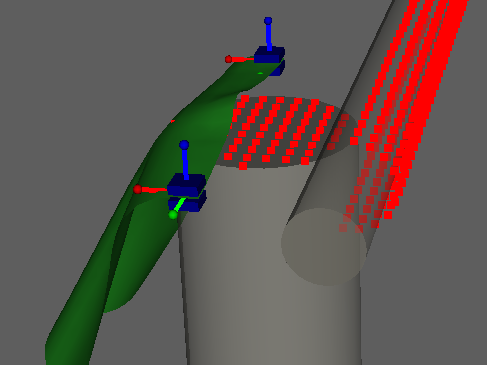
\includegraphics[width=.45\linewidth]{cloth_wafr}\hfill
    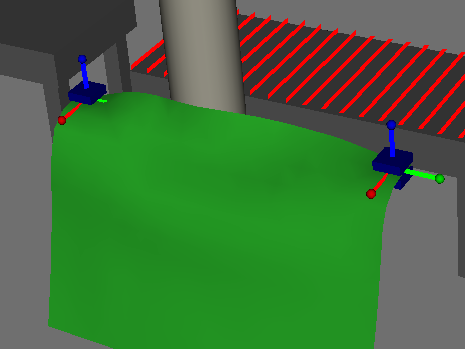
\includegraphics[width=.45\linewidth]{cloth_single_pole}%
    \caption{Initial state of the four experiments, where the red points act as attractors for the deformable object.}
    \label{fig:experimental_setup_scene}
\end{figure}


\begin{figure}[t]
    \centering
    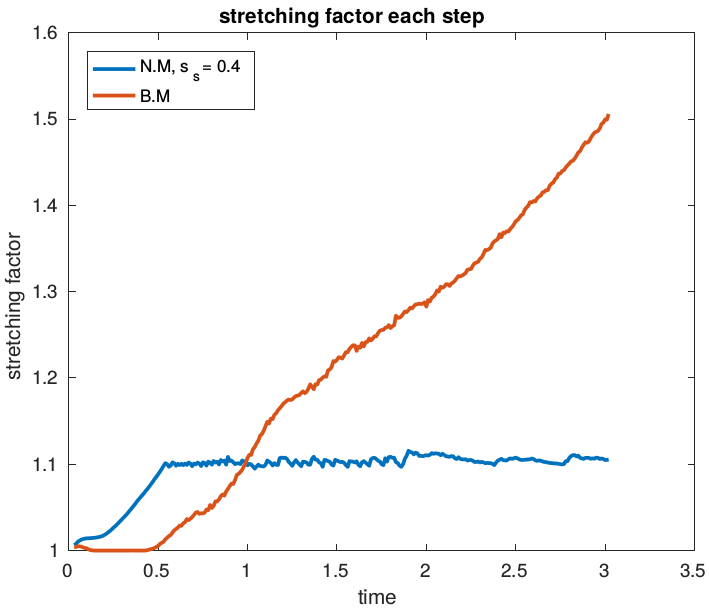
\includegraphics[width=.45\linewidth]{stretching_rope_cylinder} \hfill
    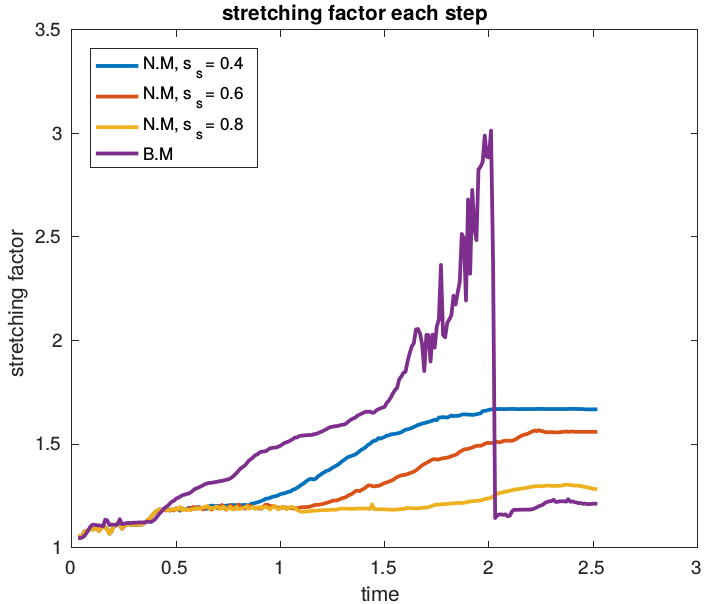
\includegraphics[width=.45\linewidth]{stretching_cloth_single_pole}%
    \caption{Cloth passing single pole}
    \label{Fig: stretching factor scene_cloth_single_pole}
    \caption{(a) The red line shows the $\stretchcurr$ of the benchmark and the blue line shows the $\stretchcurr$ of the new controller with $s_s = 0.4$ throughout the simulation. (b) The purple line shows the $\stretchcurr$ of the benchmark, and the blue, red, and yellow lines each show the $\stretchcurr$ of the new controller with $s_s = 0.4$, $s_s = 0.6$, and $s_s = 0.8$, respectively.}
    \label{fig:experiment_stretching_factorFig: experiment_stretching_factor}
\end{figure}




%We find that setting a tighter constraint, such as increasing the value of $s_s$, can help prevent excessive stretching in the object, as shown in Fig. \ref{Fig: cos_stretching}. 


% Explain the trade-off between constraints avoidance and control accuracy
%Examining Fig. \ref{Fig: experiment_model_error} and Fig. \ref{fig:experiment_stretching_factorFig: experiment_stretching_factor}, we found that when there is no constraints violation detected, the new controller can generally have a smaller control error.
%When the constraints violation happens, the new controller will tend to mitigate this violation and take the trade off in control accuracy.  



\subsection{Controller Task Performance} \label{Results:Controller Task Performance}

Besides the quantitative analysis of the model accuracy and stretching avoidance, we ran another two experiments, rope-matching-zig-path and cloth-covering-two-cylinder, one each with the rope or the cloth, as shown in Fig.~\ref{fig:experimental_setup_scene} to see how the new method performed for some coverage tasks. Both the benchmark and the new controllers are able to perform these tasks with comparable performance; reaching approximately the same configurations when forward progress stops due to a local minimum (Fig.~\ref{fig:cloth_wafr_performance}), and completing the task (Fig.~\ref{fig:zigzeg_performance}). This result suggests that we have not lost functionality with respect to the benchmark despite changing the model and control method used.


\begin{figure}[t]
    \centering
    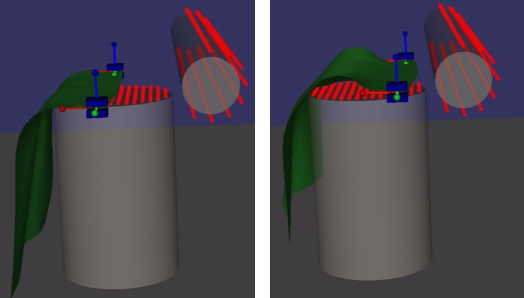
\includegraphics[width=\columnwidth]{cloth_wafr_performance.png}
    \caption{Cloth-covering-two-cylinder task start and end configurations. Both controllers are unable to make progress due to a local minima.}
    \label{fig:cloth_wafr_performance}
\end{figure}


\begin{figure}[t]
    \centering
    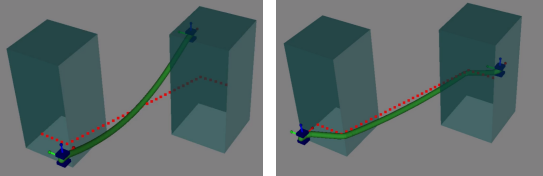
\includegraphics[width=\columnwidth]{zigzeg_performance.png}
    \caption{Rope-matching-zig-path start and end configurations. Both controllers are able to succeed at the task, bringing the rope into alignment with the desired path.}
    \label{fig:zigzeg_performance}
\end{figure}



\subsection{Physical Robot Experiments}

To evaluate our new model and controller on a physical system, we set up an experiment with cloth-like objects manipulated by two 7DoF KUKA iiwa arms (Fig.~\ref{fig:physical_experiment_screenshots_ctl}). To sense the position of the cloth, we use the AprilTags~\cite{olson2011tags} and IAI Kinect2~\cite{iai_kinect2} libraries. The parameters are set as $\drkdir = 4$, $\drkdist = 10$, $\drkrot = 10$ for the new model, $l_c = 0.08$, and $s_s = 0.6$ for the new controller. We set up a task similar to the cloth-passing-single-pole example using a paper towel. For this task, the baseline controller tears the paper towel while the new controller avoids excessive overstretch, instead wrapping around the pole to reach a local minimum.

\begin{figure}[t]
    \centering
    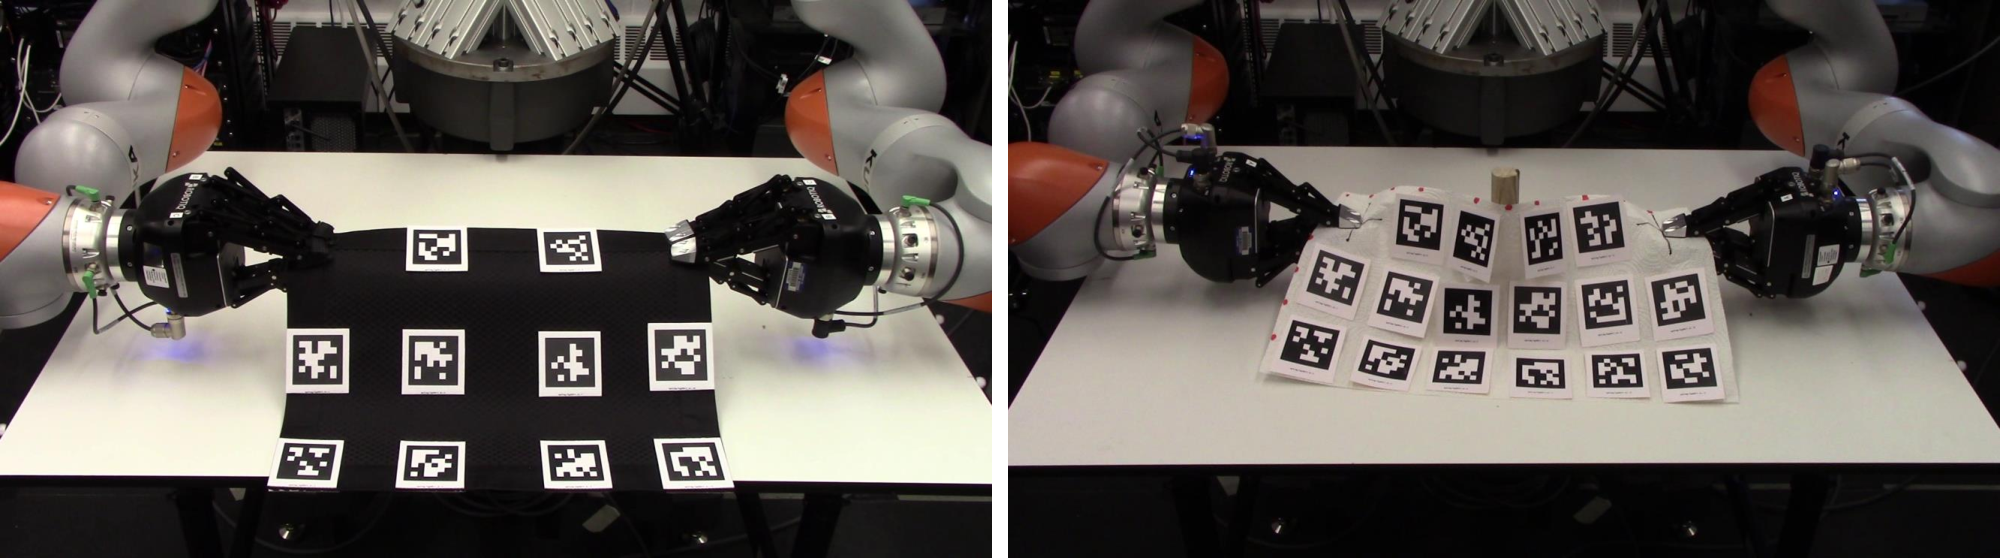
\includegraphics[width=0.85\columnwidth,trim=6.7in 0 0 0,clip]{physical_robot_experiment_screenshots.pdf}
    \caption{Initial setup for the physical robot stretching avoidance test.}
    \label{fig:physical_experiment_screenshots_ctl}
\end{figure}


\subsection{Computation Time}


\begin{table}[t]
%\renewcommand{\arraystretch}{1.2}
\centering
\resizebox{\linewidth}{!}{
\begin{tabular}{|c|c|c|c|c|}
\hline
        & rope-wrapping & rope-matching & cloth-passing & cloth-wrapping \\
        & -cylinder     & -zig-path     & single-pole   & -two-cylinders \\ \hline
BM       & 0.0055   & 0.0054  & 0.0153  & 0.0037   \\ \hline
NM       & 0.0342   & 0.0834  & 0.2363  & 0.1008   \\ \hline
\end{tabular}
}
\caption{Mean computation time (s) to compute the gripper motion for a given state. BM: benchmark method; NM: new method.}
\label{tbl:constraint_controller_time_report}
\end{table}



To verify the practicality of our method, we gathered data comparing its computation time to the benchmark's and to using the Bullet simulator. Table~\ref{tbl:constraint_controller_time_report} shows the average computation time of a call to the controller for the new method vs. the benchmark. As expected, the benchmark, which uses a linear model, is faster than the new method. However, the computation times for the new method are still reasonable to use in a control loop.

